% question 10
\qs{}{
    Whose family has the least amount of money left after paying total school fees?
}

The base \texttt{view} serves as the central hub of all the information needed. It has the main price of their tuition fee, including miscellaneous and laboratory fees, the price of their course given that it's been multiplied to the price per unit of their college, as well as the income of their family.

the \texttt{courseTotals} aggregates all the price of the courses taken by each student, the \texttt{sum()} function was grouped accordign to the \texttt{stud\_id} of each row. 

\texttt{deducts} then calculates the total deductions and the remaining money of each family in the record. In this view, querying for the least amount of money left is possible by using the \texttt{min()} function to match the lowest record.
\vspace{\baselineskip}

\sol{}
\noindent\line(1, 0){0.89\linewidth}
\begin{verbatim}
create view base as
select en.stud_id, en.crs_id, (en.enr_tuition_fee + en.enr_misc_fee + en.enr_lab_fee)
as mainPrice, (en.enr_ppu * course.crs_units) as coursePrice, student.stud_fam_income
as income from enrollment en
join course on en.crs_id = course.crs_id
join student on en.stud_id = student.stud_id
group by en.crs_id;

create view courseTotals as
select stud_id, mainPrice, sum(coursePrice) as totals, income from base group by stud_id;

create view deducts as
select stud_id, (income - (mainPrice + totals)) as money from courseTotals;

select concat(student.stud_fname, " ", student.stud_lname) as Name, money from deducts 
join student on deducts.stud_id = student.stud_id
where money = (select min(money) from deducts);
\end{verbatim}
\noindent\line(1, 0){\linewidth}

\begin{figure}[H]
    \centering
    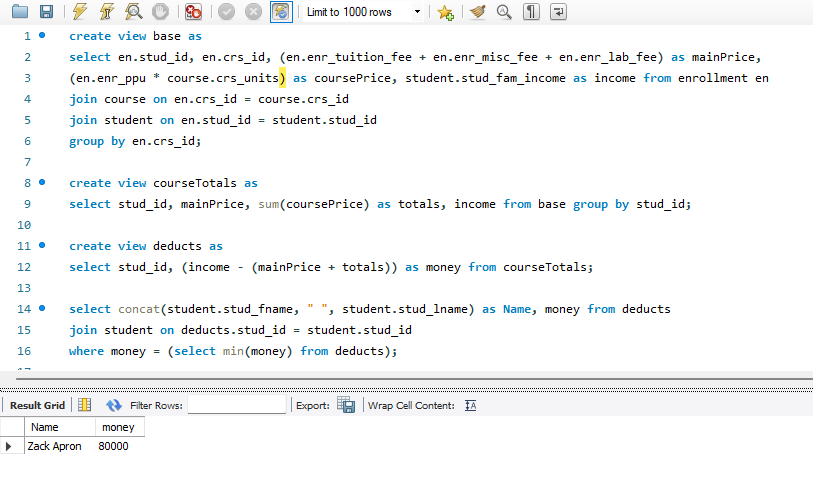
\includegraphics[width=0.7\linewidth]{images/q10.png}
    \caption{Question 10 Query and Output}
\end{figure}
